
當接受了某些數據共享即將發生的事實,就必須接受對共享數據的同步。記住,在沒有同步的情況下,對相同數據的併發訪問都會導致數據競爭和未定義行為。

保護共享數據的常用方法是使用互斥鎖:

\begin{lstlisting}[style=styleCXX]
std::mutex m;
size_t count;// Guarded by m
… on the threads …
{
	std::lock_guard l(m);
	++count;
}
\end{lstlisting}

這裡使用C++17模板類型推斷來實現\texttt{std::lock\_guard}。在C++14中,必須指定模板類型實參。

使用互斥對象相當簡單,訪問共享數據的代碼都應該位於臨界區,也就是在鎖定和解鎖互斥對象的調用之間。互斥鎖的實現有正確的內存柵欄,以確保臨界區中的代碼不會被硬件或編譯器移出臨界區(編譯器通常不會在鎖操作中移動代碼。不過,只要遵循內存柵欄的語義,理論上可以做這樣的優化)。

這時候通常會問的是:“互斥鎖的開銷有多大?”然而,這個問題並沒有很好地答案:對於特定的硬件和給定的互斥鎖實現,當然可以給出絕對的答案,甚至以納秒為單位,但是這個值有什麼意義呢?這當然比沒有互斥對象開銷小得多,但沒有互斥對象,結果就會不正確(而且有更簡單的方法可以快速生成不正確的程序)。所以,“開銷大”的定義只能與替代方案相比較,這自然引出了下一個問題,替代方案是什麼?

最明顯的替代方法是使計數原子化:

\begin{lstlisting}[style=styleCXX]
std::atomic<size_t> count;
… on the threads …
++count;
\end{lstlisting}

還必須考慮需要什麼內存序來與計數上的操作相關聯。如果稍後使用該計數,例如在數組中進行下標索引,那可能需要釋放-獲取序。但如果只是一個計數,只是要統計一些事件並報告數量,那就不需要內存序限制:

\begin{lstlisting}[style=styleCXX]
std::atomic<size_t> count;
… on the threads …
count.fetch_add(1, std::memory_order_relaxed);
\end{lstlisting}

是否使用柵欄取決於硬件。在x86上,原子增量指令有“內置”的雙向內存柵欄,自由序不會讓它更快。儘管如此,為了可移植性和清晰性,指定代碼需要的內存序仍然很重要。記住,\textbf{寫代碼不是給解析代碼的編譯器看的,而是給需要閱讀代碼的其他開發者看的}。

具有原子增量的程序沒有鎖,也不需要任何鎖。然而,它依賴於特定的硬件能力。處理器有一個原子增量指令,這類指令的集合相當小。如果需要一個沒有原子指令的操作,該怎麼辦?在C++中,沒有原子乘法(不知道任何硬件有這樣的能力。當然,在x86、ARM或其他任何通用CPU架構上都找不到)。

不過,有一種“通用的”原子操作,可以用來構建任何讀-改-寫操作(困難程度不同)。這個操作稱為\textbf{比較-交換},在C++中稱為\texttt{compare\_exchange}。它有兩個參數:第一個是原子變量的預期當前值,第二個是預期的新值。如果實際的當前值與期望值不匹配,則什麼也不會發生,原子變量也不會發生更改。但是,如果當前值與期望值匹配,則需要的值將寫入原子變量。C++的\texttt{compare\_exchange}操作會返回true或false來指示寫操作是否發生(如果發生則返回true)。如果變量與預期值不匹配,則在第一個參數中返回實際值。通過比較和交換,可以實現原子增量操作:

\begin{lstlisting}[style=styleCXX]
std::atomic<size_t> count;
… on the threads …
size_t c = count.load(std::memory_order_relaxed);
while (!count.compare_exchange_strong(c, c + 1,
	std::memory_order_relaxed, std::memory_order_relaxed)) {}
\end{lstlisting}

首先,C++中操作的實際名稱是\texttt{compare\_exchange\_strong}和\texttt{compare\_exchange\_weak}。不同的是,即使當前值和期望值匹配,弱版本有時也會返回false(在x86上,這沒有區別,但在一些平臺上,弱版執行的更快)。其次,該操作接受兩個內存序:第二個內存序應用於比較失敗時(因此它只是操作的比較部分的內存順序),第一個內存序應用於比較成功併發生寫操作時。

分析這個實現是如何工作的。首先,以原子的方式讀取count的當前值\texttt{c}。當然,增量後是\texttt{c + 1},但不能直接將其賦給count。因為在讀取之後,更新之前,另一個線程也可以給count賦值。因此,必須進行條件寫入:如果count的當前值仍然是\texttt{c},則將其替換為所需的值\texttt{c + 1}。否則,用新的當前值更新\texttt{c}(\texttt{compare\_exchange\_strong}可以做到),然後再試一次。只有捕捉到原子變量,在上次讀取的時間和試圖更新之間沒有變化時,循環才會退出。當然,有原子增量操作時,就沒有理由這樣來增加計數。但這種方法可以推廣到其他計算中,可以使用其他表達式,而不是\texttt{c + 1},並且程序將以同樣的方式進行。

雖然這三個版本的代碼都執行相同的操作,但它們之間有著根本性的區別,必須對此進行更詳細的研究。

\subsubsubsection{6.3.1\hspace{0.2cm}鎖、無鎖和無等待}

使用互斥鎖是最容易理解的,一個線程可以持有鎖,因此線程可以增加計數。當釋放鎖後,另一個線程可以獲取它並增加計數,依此類推。最多隻能有一個線程持有鎖並進行操作,所有需要訪問的剩餘線程都在等待該鎖。但是,即使擁有鎖的線程也不能保證可以正常運行。如果需要在完成任務之前訪問另一個共享變量,那麼可能需要等待由其他線程持有的鎖。這是常見的基於鎖的方式,通常不是最快的,但最容易理解。

第二種方式與第一種非常不同,進行原子增量操作的線程會毫不延遲地執行。當然,硬件本身必須鎖定對共享數據的訪問,以確保操作的原子性(這是通過一次對整個緩存線的獨佔訪問,並授予一個處理器來實現的)。從開發者的角度來看,這種獨佔訪問表明其本身會增加執行原子操作所需的時間。然而,代碼本身沒有等待,沒有嘗試和再嘗試。這種程序稱為\textbf{無等待}。在一個無等待程序中,所有線程都能正常運行,在任何時候都在執行操作(儘管線程之間為了訪問同一個共享變量而發生爭用,有些操作可能會花費更長的時間)。無等待的實現通常只適用於非常簡單的操作(例如增加計數),但只要有這種實現,可能會比基於鎖的實現更簡單。

最後一個方式理解起來有些困難。這裡沒有鎖,但有一個循環重複了未知的次數。這裡的實現的功能類似於鎖,任何等待鎖的線程也會困在一個類似的循環中,不停的嘗試獲得鎖。二者的關鍵的區別在於,基於鎖的程序中,當一個線程獲取鎖失敗,必須再次嘗試時,可以推斷其他線程擁有鎖。不能確定線程是否會很快釋放鎖,或者其工作有什麼進展(例如,可能正在等待用戶輸入一些東西)。在基於比較-交換的程序中,線程無法更新共享計數的唯一原因是其他線程先進行了更新。因此,在所有試圖同時增加計數的線程中,至少有一個是成功的。這種程序稱為\textbf{無鎖}程序。

我們已經瞭解了併發程序主要的三種類型:

\begin{itemize}
\item 
無等待的程序中,每個線程都在執行必要的操作,並且總是朝著最終目標前進。不需要等待訪問,也不需要重做任何工作。

\item 
無鎖程序中,多個線程可能會更新相同的共享數據,但只有一個會成功。其餘的將放棄基於原始值所做的工作,讀取更新後的值,並再次進行計算。但至少有一個線程總是保證提交它的工作,而不必重做。因此,儘管不一定是全速前進,但整個程序是在前進的。

\item 
基於鎖的程序中,線程持有使其能夠訪問共享數據的鎖。但是,僅因為持有鎖並不意味著會對這些數據做什麼。因此,當併發訪問發生時,最多隻有一個線程在有進展,但這也無法保證。
\end{itemize}

理論上講,這三個程序之間的區別很明顯。但讀者想知道,哪個版本更快?可以在谷歌基準測試中運行每個版本的代碼。例如,下面是基於鎖的版本:

\hspace*{\fill} \\ %插入空行
\noindent
\textbf{01\_sharing\_incr\_mbm.C}
\begin{lstlisting}[style=styleCXX]
std::mutex m;
size_t count = 0;
void BM_lock(benchmark::State& state) {
	if (state.thread_index == 0) count = 0;
	for (auto _ : state) {
		std::lock_guard l(m);
		++count;
	}
}
BENCHMARK(BM_lock)->Threads(2)->UseRealTime();
\end{lstlisting}

必須在線程之間共享的變量在全局作用域中聲明。初始設置(如果有的話)可以限制為一個線程,其他基準也類似,只有測試的代碼發生了變化。下面是結果:

%\hspace*{\fill} \\ %插入空行
\begin{center}
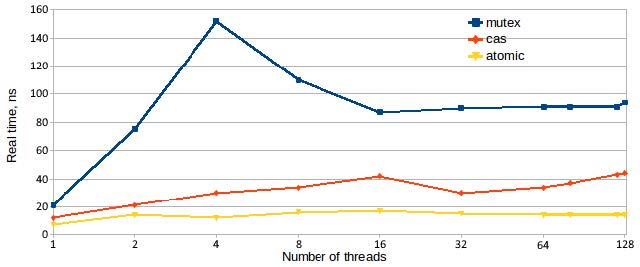
\includegraphics[width=0.9\textwidth]{content/2/chapter6/images/1.jpg}\\
圖6.1 - 共享計數增量的性能:基於互斥鎖、無鎖(比較-交換,或CAS)和無等待(原子)
\end{center}

這裡唯一想不到的結果是,基於鎖的版本的性能非常差。然而,這只是一個數據點,並不是全部。特別是,雖然所有互斥對象都是鎖,但並不是所有的鎖都是互斥對象。可以嘗試提出一種更有效的鎖實現(至少,以滿足我們的需求)。

\subsubsubsection{6.3.2\hspace{0.2cm}不同的問題使用不同的鎖}

標準的C++互斥鎖在保護對共享變量的訪問時性能非常差,特別是當有很多線程在同一時間修改這個變量時(如果所有線程都在讀取這個變量,根本不需要保護,併發只讀訪問不會導致數據競爭)。但是,鎖的效率低下是因為實現,還是因為鎖本身存在問題?根據前一章的瞭解,可以預期鎖的效率都比原子遞增計數器低,這是因為基於鎖的方案會使用兩個共享變量(鎖和計數),而原子計數器只使用一個共享變量。然而,操作系統提供的互斥對象對於鎖定非常短的操作(比如計數增量)通常不是特別有效。

對於這種情況,最簡單有效的鎖就是自旋鎖。自旋鎖的思想是:鎖本身只是一個可以有兩個值的標誌,比如0和1。如果flag值為0,表示不鎖定。看到這個值的線程都可以將標誌設置為1並繼續。當然,讀取標誌並將其設置為1的整個操作必須是原子操作。任何看到值為1的線程都必須等待,直到該值變回0,以表明鎖可用。最後,當一個將標誌從0更改為1的線程準備釋放鎖時,將把值更改回0。

鎖實現的代碼如下所示:

\begin{lstlisting}[style=styleCXX]
class Spinlock {
	public:
	void lock() {
		while (flag_.exchange(1, std::memory_order_acquire)) {}
	}
	void unlock() { flag_.store(0, std::memory_order_release); }
	private:
	std::atomic<unsigned int> flag_;
};
\end{lstlisting}

代碼中,只展示了鎖定和解鎖函數。類還需要默認構造函數(原子整數在其自己的默認構造函數中初始化為0),以及使其不可複製的聲明。

注意,鎖定標誌不使用條件交換,而總是將1寫入標誌。原因是,如果標誌的原始值是0,交換操作將設置為1並返回0(循環結束),這就是我們想要的。但是如果原來的值是1,就被1代替,也就是不發生改變。

另外,注意兩個內存柵欄:鎖定伴隨著獲取柵欄,解鎖伴隨著打開柵欄。柵欄劃分了臨界區,並確保在\texttt{lock()}和\texttt{unlock()}調用之間的代碼都留在那裡。

讀者可能想看這個鎖與標準互斥鎖的基準比較,但是我們不打算展示:這個自旋鎖的性能非常糟糕。為了使它有用,需要一些優化。

首先,如果標誌的值是1,實際上不需要用1替換它,可以不去管它。為什麼這很重要?交換是一個讀-改-寫操作。即使它將舊的值更改為相同的值,也需要獨佔訪問包含該標誌的緩存行,這裡不需要獨佔訪問來讀取該標誌。這在以下場景中很重要,一個鎖鎖住了,擁有鎖的線程沒有更改它(正在忙著做它的工作),但是其他線程都在檢查鎖,並等待鎖的值更改為0。如果線程不嘗試寫入標誌,那麼緩存行就需要在CPU之間切換,線程在緩存中都有相同的內存副本,並且這個副本是當前的,不需要發送數據到其他地方。只有當其中一個線程實際修改了值時,硬件才需要將內存中的新內容發送給所有的CPU。下面是我們剛剛描述的優化,以代碼的形式完成:

\begin{lstlisting}[style=styleCXX]
class Spinlock {
	void lock() {
		while (flag_.load(std::memory_order_relaxed) ||
		flag_.exchange(1, std::memory_order_acquire)) {}
	}
}
\end{lstlisting}

這裡的優化是,首先讀取該標誌,直到看到0,然後將其與1交換。如果另一個線程先獲得了鎖,那麼在進行檢查和交換之間,這個值可以變成1。另外,在預檢查標誌時,不去關心內存柵欄,因為最終的決定性檢查會使用交換和內存柵欄來完成。

即使進行了這種優化,鎖的性能仍然很差。原因與操作系統傾向於優先處理線程的方式有關。當一個線程正在做一些有用的事情,那麼將會獲得更多的CPU時間。但在我們的例子中,計算量最大的線程是在等待標誌改變的同時,查詢獲得標誌線程的狀態。這可能會導致一種不希望出現的情況,即一個線程試圖獲得鎖並將CPU分配給它,而另一個線程希望釋放鎖,但在一段時間內沒有調度執行。解決方案是等待的線程在多次嘗試後放棄CPU,這樣其他線程就可以運行,並且可以完成自己的工作並釋放鎖。

有幾種方法可以讓線程釋放對CPU的控制,沒有一個通用的最好的方法,大多數都是通過系統函數調用完成的。在Linux上,通過調用\texttt{nanosleep()}在很短的一段時間內(1納秒)調用\texttt{sleep},可能會產生最好的結果,通常比調用\texttt{sched\_yield()}更好,\texttt{sched\_yield()}是另一個提供CPU訪問的系統函數。與硬件指令相比,所有的系統調用開銷都很大,所以最好不要頻繁使用。當嘗試幾次獲取鎖後,將CPU交給另一個線程,然後再嘗試時,就達到了最佳的平衡:

\hspace*{\fill} \\ %插入空行
\noindent
\textbf{01c\_spinlock\_count.C}
\begin{lstlisting}[style=styleCXX]
class Spinlock {
	void lock() {
		for (int i=0; flag_.load(std::memory_order_relaxed) ||
		flag_.exchange(1, std::memory_order_acquire); ++i) {
			if (i == 8) {
				lock_sleep();
				i = 0;
			}
		}
	}
	void lock_sleep() {
		static const timespec ns = { 0, 1 }; // 1 nanosecond
		nanosleep(&ns, NULL);
	}
}
\end{lstlisting}

釋放CPU之前,獲取鎖的最佳嘗試次數取決於硬件和線程數。一般來說,8到16之間比較合適。

現在,已經準備好進行第二輪的基準測試了,結果如下:

%\hspace*{\fill} \\ %插入空行
\begin{center}
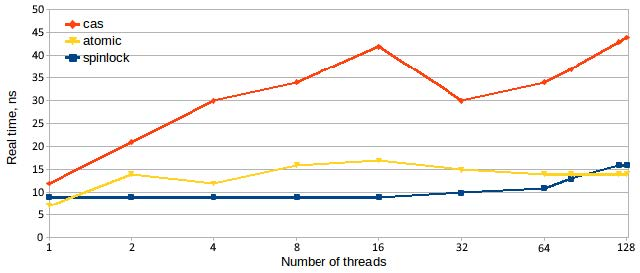
\includegraphics[width=0.9\textwidth]{content/2/chapter6/images/2.jpg}\\
圖6.2 - 共享計數增量的性能:基於自旋鎖、無鎖(比較-交換,或CAS)和無等待(原子)
\end{center}

自旋鎖已經做得很好了,性能明顯優於比較-交換實現,並可以與無等待操作進行競爭。這裡會有兩個問題:首先,如果自旋鎖的速度快得多,為什麼不都使用自旋鎖?其次,如果自旋鎖這麼好,為什麼還需要原子操作(當然,除了鎖實現的原子操作)?

第一個問題的答案可以歸結為本節的標題,不同的問題使用不同的鎖。自旋鎖的缺點是等待的線程不斷地使用CPU或“忙等待”。另一方面,等待系統互斥的線程大部分是空閒的(休眠)。如果需要等待幾個週期,即增量操作的持續時間,那麼忙碌等待也不錯,比讓線程進入睡眠狀態要快得多。另一方面,如果鎖定的計算包含多個指令,那麼等待自旋鎖的線程將浪費大量CPU時間,並剝奪其他工作線程訪問所需的硬件資源的機會。總的來說,C++的互斥量(\texttt{std::mutex})或OS的互斥量通常會進行平衡,鎖定一條指令的效率有點低,鎖定一個需要幾十納秒的計算是可以的。如果需要持有鎖很長時間(長是相對的,處理器很快,所以1毫秒是非常長的),這就打敗了另一種選擇。已經討論了極端性能(以及極端實現性能的努力),因此大多數HPC開發者要麼實現自己的快速鎖來保護短計算,要麼使用現成的庫。

第二個問題,“鎖還有其他的缺點嗎?”讓我們帶著這個問題進入下一節。

\subsubsubsection{6.3.3\hspace{0.2cm}鎖的和無鎖的區別}

在討論無鎖編程的好處時,第一個點是“更快”。但這並不一定,如果針對特定的任務進行優化,鎖的實現可以非常高效。但是,基於鎖的方法還有其他缺點,不過這些缺點不依賴於實現。

最頭痛的是可能出現死鎖。當程序使用多個鎖時,就會發生死鎖,比如lock1和lock2。線程A擁有lock1,需要獲取lock2。線程B已經擁有了lock2,需要獲取lock1。兩個線程都不能繼續,而且都將永遠等待,因為唯一可以釋放它們所需鎖的線程被鎖阻塞了。

如果同時獲得兩個鎖,總是以相同的順序獲得鎖,就可以避免死鎖。C++有一個用於此目的的函數\texttt{std::lock()}。但通常不能同時獲得鎖,當線程A獲得lock1時,無法知道我們也需要lock2,因為該信息隱藏在由lock1保護的數據中。我們將在下一章討論併發數據結構時看到一些例子。

如果不能獲取多個鎖,也許解決方案會嘗試獲取。然後,若不能獲得所有的鎖,那麼釋放已經持有的鎖,以便其他線程可以獲得。在我們的例子中,線程A持有lock1,它也會嘗試獲得lock2,但不會阻塞。大多數鎖都有\texttt{try\_lock()},要麼獲得鎖,要麼返回false。後一種情況下,線程A釋放lock1並試圖再次鎖定它們。這可能行得通,特別是在一個簡單的測試中。但它自己也有危險,當兩個線程不斷地傳遞鎖時,就會出現活鎖。線程A有lock1,但沒有lock2,線程B有lock2,放棄了它,得到了lock1,現在它不能再得到lock2了,因為線程A擁有了lock2。有一些算法可以獲取多個鎖,從而保證最終成功。但這可能要需要很長一段時間,並且算法也相當複雜。

解決多個鎖的問題是互斥對象不能組合,不能將兩個或多個鎖組合成一個。

即使沒有活鎖和死鎖的危險,基於鎖的程序也會遇到其他問題。其中較為頻繁和難以診斷的一種稱為協同。可以在多個鎖中發生,也可以只在一個鎖中發生。協同看起來是這樣的:假設有一個鎖保護的計算。線程A目前擁有這個鎖,並且正在對共享數據進行操作,其他線程正在等待。然而,這項工作並不是一次性的,每個線程都有許多任務要做,每個任務的一部分需要獨佔訪問共享數據。線程A完成一個任務,釋放鎖,然後快速切換到下一個任務,直到它再次需要鎖。鎖釋放了,其他線程都可以獲得,但其他線程沒完全醒,而線程A在CPU上,並沒有睡。因此,線程A再次獲得鎖,只是因為競爭對手還沒有做好準備。線程A的任務像車隊中的卡車一樣快速執行,而其他線程什麼也做不了。

鎖的另一個問題是,沒有優先級的概念。持有鎖的低優先級線程可以搶佔需要相同鎖的高優先級線程。因此,高優先級線程必須等待低優先級線程決定的時間,這種情況似乎與高優先級的概念不一致,這種情況有時稱為優先級倒置。

既然已經理解了鎖的問題並不侷限於性能,那麼看看無鎖程序在相同的複雜性下會有怎樣的表現。首先,在無鎖程序中,至少有一個線程不被阻塞。最壞的情況是,當所有線程同時執行比較-交換(CAS)操作,並且原子變量的期望與當前值相同時,其中一個線程將看到期望值(因為唯一可以更改的方法是通過CAS操作)。其他線程將放棄它們的計算結果,重新加載原子變量,並重復計算,但是在CAS上成功的線程可以移動到下一個任務,這避免了死鎖的可能性。如果排除了死鎖和避免死鎖的嘗試,也就不必擔心活鎖。由於所有線程都忙於計算通向原子操作(如CAS)的路徑,高優先級線程更有可能最先到達那裡,並提交其結果,而低優先級線程更有可能使CAS失敗,並重做其工作。類似地,提交結果的一次成功並不會使“獲勝”的線程比所有其他線程有任何優勢,準備先嚐試執行CAS的線程就是成功的線程。這自然就消除了出現協同的可能。

無鎖編程有什麼不好呢?有兩個主要的缺點。第一個是其優點的反面,即使CAS嘗試失敗的線程也會保持忙碌。這解決了優先級問題,但代價很高。在高爭用的情況下,大量的CPU時間會浪費在重複工作上。更糟糕的是,這些為訪問單個原子變量而競爭的線程,會從進行一些不相關計算的其他線程那裡奪取CPU資源。

第二個缺點性質完全不同。雖然大多數併發程序都不容易編寫或理解,但無鎖程序的正確設計和實現都非常困難。基於鎖的程序只需要保證構成單個邏輯事務的操作集都在鎖下執行。當存在多個邏輯事務時,例如(而不是所有)共享數據對幾個不同的事務來說是公共的,這就更難了。這就是提出多鎖問題的原因。儘管如此,推斷基於鎖的正確性並不是那麼困難。如果代碼中有一段共享數據,就必須指明哪個鎖保護該數據,並證明沒有線程可以在不先獲取該鎖的情況下訪問該數據。如果不是這樣,那麼就會出現數據競爭。如果滿足了這些需求,就不會出現數據競爭(可能會出現死鎖和其他問題)。

另一方面,無鎖程序有無限多種數據同步方案。因為沒有線程會暫停,所以無論線程執行原子操作的順序如何,結果都必須是正確的。此外,如果沒有明確的臨界區,就得擔心內存序和程序中所有數據的可見性,而不僅僅是原子變量。這裡必須問問自己,有沒有可能因為內存順序要求不夠嚴格,一個線程可以更改數據,而另一個線程可以看到這個數據的舊版本?

解決複雜性問題的通常方法是模塊化和封裝。將複雜的代碼收集到模塊中,每個模塊都有一個定義良好的接口和一組明確的需求和保證,主要關注實現各種併發算法的模塊。不過本書會有一個不同的方向,本章的其餘部分將專門討論適用於併發的數據結構。




































